\section{The Testradius}
\index{Testradius}
\begin{figure}[h]
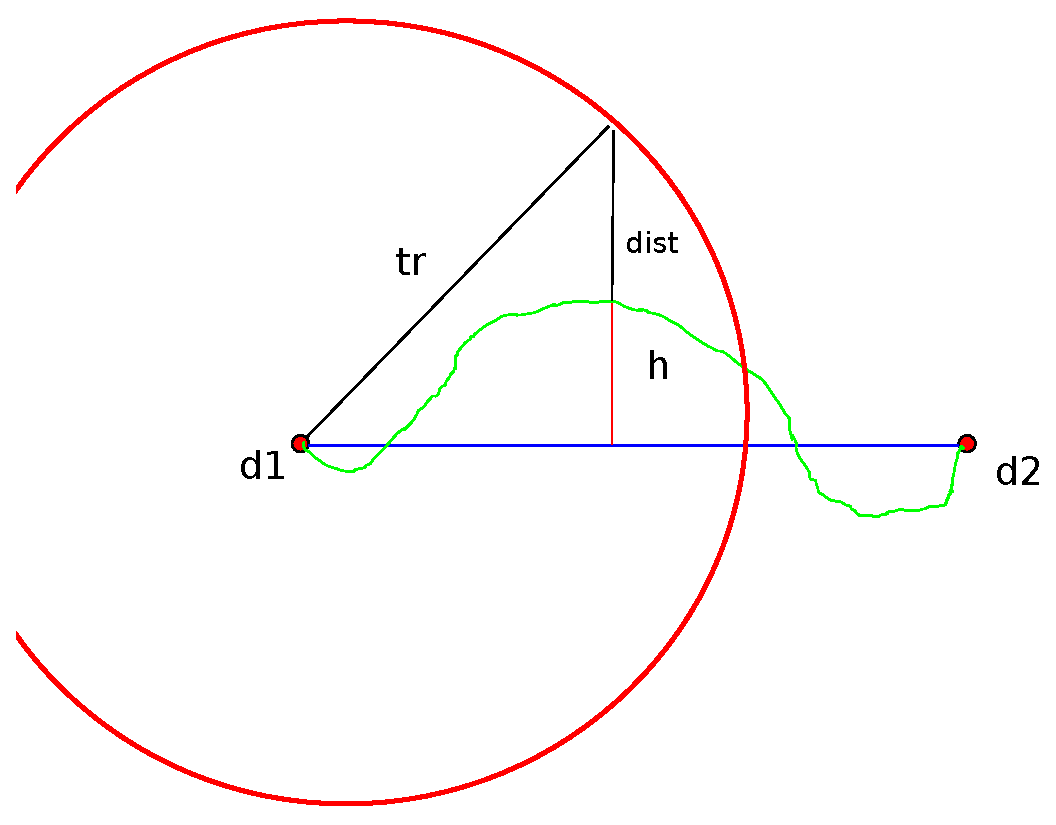
\includegraphics[scale=0.5]{images/03.06.testradius.eps}
\caption{Testradius $t_r$ must be large enough so that it covers any deflection $h$ \emph{plus} the user 
	 defined distance $dist$.
	}
\end{figure}

Summing up the results of the preceeding section, we now present formulas for calculating the 
test radius $t_r$.

We now consider two DRs $d_1$ and $d_2$ connected by a path $P$, with the distance from $d_1$ to $d_3$ beeing
$d$ along $P$ and $\tilde{d}$ in direct line. 
Assume further that P has a deflection $h$. By convexity we can assume this deflection to appear at the middle
of the line segment between $d_1$ and $d_2$. I.e: if the radius is large enough to cover the deflection
in the middle of the line segment, this deflection will be covered anywhere else.

Now the testradius $tr$ around $d_1$ must be large enough to cover a distance of $h+dist$ at a distance of $\frac{\tilde{d}}{2}$
from $d_1$.  The Phythagorean Theorem then gives the condition:
\index{Testradius!Condition for valid testradius} 
\begin{equation}
\label{testradius_condition}
 t_r^2  \geq \left(\frac{\tilde{d}}{2}\right)^2 + \left(h+dist\right)^2
\end{equation}

Condition \ref{testradius_condition} can be fulfilled with equality by choosing a radius $t_{r}$ as the square root of the right side:
\index{Testradius!Exact testradius tr}

\begin{equation}
 \label{testradius_general}
 t_r  := \sqrt{\left(\frac{\tilde{d}}{2}\right)^2 + \left(h+dist\right)^2}
\end{equation}

In practical application, it may turn out to be too tedious to calculate the exact deflection $h$ of 
the path $P$, so we can estimate the exact value $h$ by the upper bound $h_{max}(\tilde{d},d)$ 
from equation \ref{HMaxOfD}. 
This yields a larger valid testradius $t_{r1}$, which also fulfills \ref{testradius_general},
and has a more simple formula:   
\index{Testradius!approximation tr1}
\begin{equation}
 \label{testradius_tr1}
  t_{r1} := \sqrt{\left(\frac{\tilde{d}}{2}\right)^2 + \left(\sqrt{ \left(\frac{d}{2}\right)^2 - \left(\frac{\tilde{d}}{2}\right)^2 }+dist\right)^2}
\end{equation}

Not subtracting the term $\left( \frac{\tilde{d}}{2}\right)^2$ in the inner square root gives another  
valid choice $tr_2$ for a testradius:   
\index{Testradius!approximation tr2}
\begin{equation}
 \label{testradius_tr2}
  t_{r2} := \sqrt{\left(\frac{\tilde{d}}{2}\right)^2 + \left(\frac{d}{2}+dist\right)^2}
\end{equation}

Finally, as $ \tilde{d}$ is bounded by $ d $, a really simple formula for a valid
testradius $t_{r3}$  can be obtained, from  \ref{testradius_tr2},  
which does not even require calculation of the direct distance $\tilde{d}$:
\index{Testradius!approximation tr3}
\begin{equation}
 \label{testradius_tr3}
 t_{r3}  := \sqrt{ \frac{1}{2}d^2 + d*dist + dist^2}
\end{equation}


